% multiple1902 <multiple1902@gmail.com>
% float.tex
% Copyright 2011~2012, multiple1902 (Weisi Dai)
% https://code.google.com/p/xjtuthesis/
% 
% It is strongly recommended that you read documentations located at
%   http://code.google.com/p/xjtuthesis/wiki/Landing?tm=6
% in advance of your compilation if you have not read them before.
%
% This work may be distributed and/or modified under the
% conditions of the LaTeX Project Public License, either version 1.3
% of this license or (at your option) any later version.
% The latest version of this license is in
%   http://www.latex-project.org/lppl.txt
% and version 1.3 or later is part of all distributions of LaTeX
% version 2005/12/01 or later.
%
% This work has the LPPL maintenance status `maintained'.
% 
% The Current Maintainer of this work is Weisi Dai.
%
\chapter{相关技术概述}
\label{RelatedChapter}

\section{命名数据网}
\par
NDN是本文的设计方案面向的基础网络架构。其主要特点是将数据,而不是地址,作为网络通信的基础,并把上层通信归纳为数据请求(Interest)和应答(Data),以名称(Name)来请求、发布对应的数据\cite{NDNRefOriginal}。以下将对该网络架构进行概述。
\subsection{综述}
\par
60年代、70年代的网络设计思路所希望解决的主要问题是资源共享,即由多个终端远程访问共享的昂贵资源,比如读卡器或是高速磁带硬盘。由此开发出的TCP/IP通信模型可以抽象为两点之间的信息交互,即服务请求方希望使用服务提供方的特定服务\footnote{来源:http://www.ccnx.org/395/1/van-jacobsen-at-google/}。因而IP报文中包含两个标识,目的地址和源地址。
\par
基于数据报交互(Packet switching)的网络架构形成的50年来,计算机及其附件变得便宜和大众化。网络所提供的方便的互联性和低存储成本使得大众对网络价值的衡量变得倾向于其所提供的数据本身,而不是数据具体存储在哪里。
\par
直接、统一的解决这一供求不对等问题的方案是用“什么”取代“哪里“,而基于数据名称而不是位置的命名数据网将是能够更好描述当今网络用户需求的网络架构模型。CCN底层并没有“端”或地址的概念,取而代之的数据的名称。然而,其设计仍然保留TCP/IP协议栈简单、健壮和可扩展的设计原则。
\par
图\ref{fig:ProtocolStacks}对比CCN和IP协议栈。
\begin{figure}[h!]
	\centering
	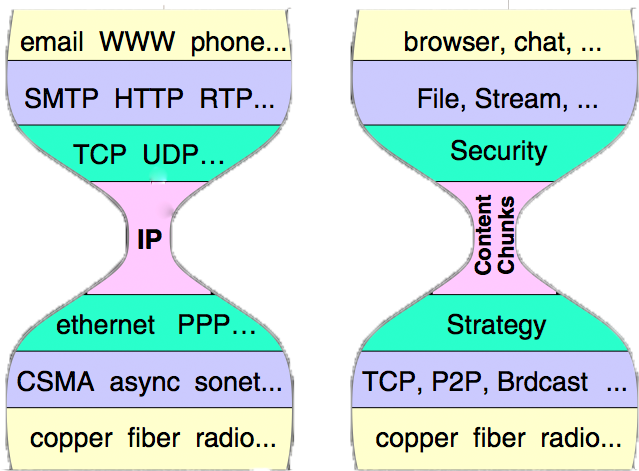
\includegraphics[width=0.5\textwidth]{NDNhourglass.png}
	\caption{TCP/IP协议栈和CCN协议栈的对比}
	\label{fig:ProtocolStacks}
\end{figure}
\par
协议栈中数层体现了两者之间的相似性,比如第二层的成帧协议体现了物理链路中发送方、接收方之间的协商;第四层传输层协议体现了数据或服务的请求者、提供者之间的协商。承上启下,为双方提供统一接口的第3层,即网络层,体现了IP协议成功的许多因素。首先,网络层对链路层提供的服务的需求很低,是无状态、不可靠、不保序、尽力而为的。CCN的网络层(即第三层),在这一点上和IP是吻合的,即不对链路层提供的服务提出过高要求。这一点为其保留了IP较多优点。同时值得一提的是,CCN也可以作为其它协议或架构的负载,包括作为IP的负载。
\par
CCN在许多关键点上不同于IP。其中两者是策略和安全。两者均为NDN协议栈中新出现的层。CCN可以最大化利用同时存在的多个连接,比如以太网、3G、蓝牙和802.11,因为CCN和第二层的关系更加简单。策略层在变化的外界条件下,根据多个同时存在的连接,做出详细的、动态的优化,从而最大化的利用多个连接。安全层保障数据本身是受信任的,而不是数据所经过的通路是受信任的,由此避免了安全策略上IP网络的许多问题。

\subsection{设计理念}
\par
CCN网络通信是由数据请求方驱使的。网络中有两种包,数据请求(Interest)和数据应答(Data)。数据请求方向本地的所有连接广播数据请求,任何收到数据请求,并且有名称满足要求的数据的节点可以应答。数据应答包的发出都是由收到特定的请求所触发,换言之,数据应答包都是为了满足特定的请求。
\par
当且仅当数据请求包的名称是数据应答包的名称的前缀子串(Name prefix)时,数据应答可以满足数据请求。CCN名称是层次结构的,所以前缀的吻合可以描述为数据应答包的名称是数据请求包的名称的子树。IP用同样的方式来解析树状的IP地址,即<网络地址,子网地址,主机地址>。IP的经验表明,这样的方式可以实现路由表树型的高效压缩和快速查找。名称前缀也是当前环境相关的。
\par
CCN节点的工作方式和IP节点是类似的:节点收到数据包,进行最长前缀匹配,并由匹配结果决定下一步行动。图\ref{fig:NodeLogic}是CCN节点模型的结构图,该图体现了一个CCN节点包含的数据结构,和在收到一个特定数据请求时进行的动作。其中主要有三个数据结构:前递表(Forwarding Information Base, FIB),数据缓存(Content Store, CS)和待应答表(Pending Interest Table, PIT),会在下文作出介绍。\cite{NDNDSRef}
\begin{figure}[h!]
	\centering
	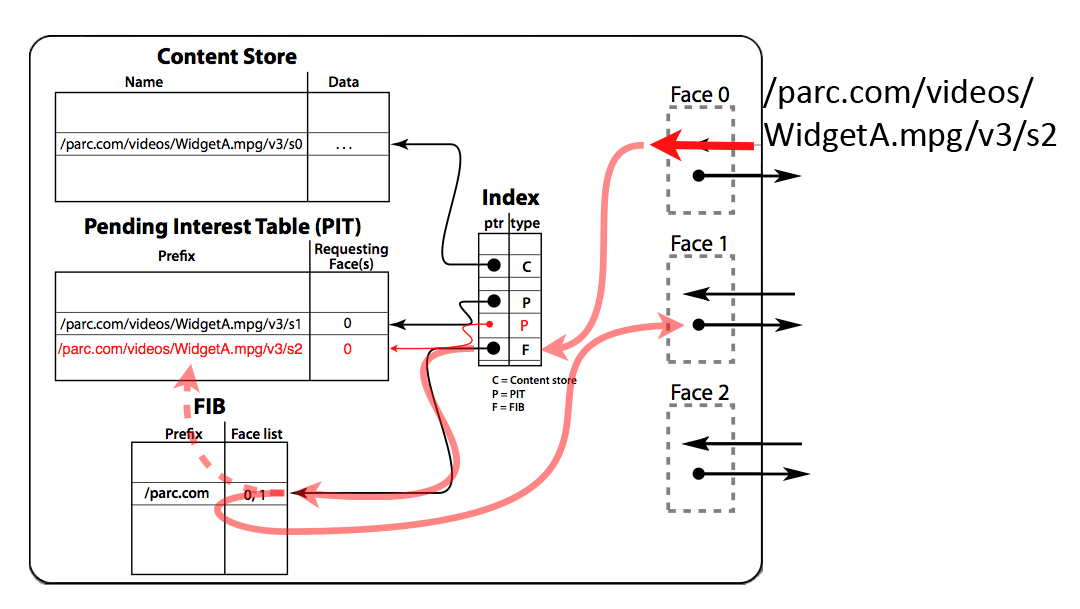
\includegraphics[width=0.9\textwidth]{CCNnodemodel.png}
	\caption{CCN节点模型}
	\label{fig:NodeLogic}
\end{figure}
\par
前递表的作用是将数据请求传递向可能有对应的数据应答的节点。其与IP的路由表相近,但是允许一个表项和多个接口进行匹配,而不是对于每一个接口,存在一张路由表。这一点体现了CCN不局限于基于一颗生成树的前递,其允许一个节点同时对多个连接的数据源进行请求,多个数据源也可以同时处理收到的请求。
\par
数据缓存和IP路由的缓存作用近似,但是替换策略不同。由于每个IP包包含了源和目的地址,其对于别的点之间的交互是不起到作用的。因此,IP路由器在将收到的包写入缓存,然后转发出去之后,就可以将该包擦除(利用最近使用(MRU)替换)。CCN包是与请求端点无关,因而每一个包有可能可以满足多个用户的数据请求,只要数据请求的名称匹配。
\par
待应答表保存了向数据提供方前递的数据请求(上行请求),因此当收到数据提供方的应答时,可以根据待应答表中的记录将数据应答传送给数据请求方。因此,在CCN中,只有数据请求包在上行时经过路由,并在经过路由节点的同时留下一系列的记录,下行的数据应答包可以根据路由节点的记录找到数据的请求者。在路由节点收到下行数据应答后,其将所收数据应答对待应答表中的对应表项中的所有节点进行多播,并且擦除该表项。长时间没有收到数据应答的数据请求会超时,而如果数据请求方仍然希望请求该数据,请求方应当负责重新发送数据请求。
\par
当数据请求包到达某节点的某接口后,节点首先进行名称的最长前缀匹配。上述数据结构的查找是有序的,数据缓存的匹配优先级高于待应答表,高于前递表。数据请求的处理逻辑如图\ref{fig:InterestLogic}所示。
\begin{figure}[h!]
	\centering
	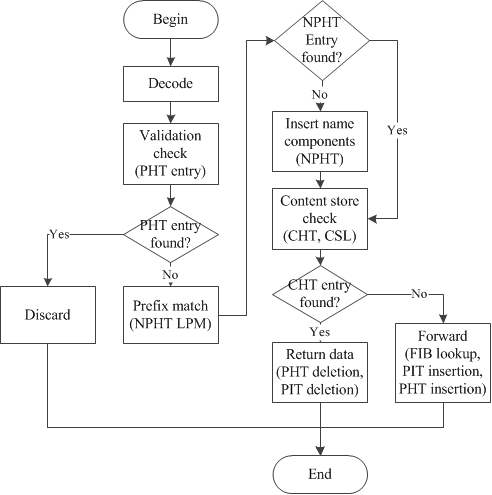
\includegraphics[width=0.75\textwidth]{InterestLogic.png}
	\caption{收到数据请求的处理逻辑}
	\label{fig:InterestLogic}
\end{figure}
\par
因此,在一个节点收到请求后,如果数据缓存找到了满足请求的数据,会直接返回该数据,同时收到的请求由于已经被满足而会被丢弃。
\par
如果数据缓存没有前缀匹配项,而待应答表中有名称完全匹配项,收到请求的接口会被加入到路由节点待应答表中该名称的下行接口表上,同时收到的请求会由于别人已经在请求同名数据,且别人的请求已经向数据源上行而被丢弃。这时路由节点所要做的只是当数据应答到来时,将数据应答也向这个数据请求的接口发送一份。
如果二者都没有匹配项,而前递表有匹配项,则数据请求根据前递表的匹配项上行。收到请求的接口将会被从前递表匹配项上移除,如果前递表匹配项此时仍不为空,则对于其所记录的每一个接口发送该数据请求。并以收到请求的接口,创建一个新的待应答表项。
\par
如果三者都没有匹配的表项,则丢弃该数据请求,因为收到请求的路由节点既没有满足要求的数据,也不知道该向哪里前递已获取满足要求的数据。
\par
数据应答包的处理要相对简单。由于数据应答包不经过路由,而是直接根据待应答表进行下行,在收到数据应答时,首先进行名称的最长前缀匹配。如果数据缓存有匹配项,则收到了重复的数据,予以丢弃。如果前递表发现了满足项,则说明待应答表中没有满足项,说明数据没有请求者,是不需要的,予以丢弃。如果带应答表中发现满足项,则(可选的)进行数据核实和写入数据缓存,之后根据待应答表的满足项移除收到数据应答的接口后,对满足项中的其它接口进行下行。
图\ref{fig:DataLogic}反映了数据应答的处理流程。不同于IP先入先出的缓存模型,CCN缓存模型允许整个网络的节点缓存实现透明缓存。所有节点可以根据自己的能力和策略进行缓存。
\begin{figure}[h!]
	\centering
	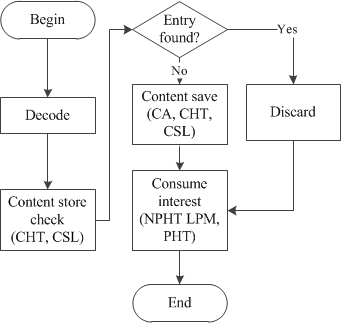
\includegraphics[width=0.50\textwidth]{DataLogic.png}
	\caption{收到数据应答的处理逻辑}
	\label{fig:DataLogic}
\end{figure}
\par
通过数据请求指定的多点数据回取的特点使得CCN在变化快速的环境下依然可以灵活应用。任何处在多个网络中的节点可以作为其所处的多个网络之间的缓存和路由。利用其缓存,一个移动的节点可以作为多个彼此不相连区域进行连接的媒介,或者为不连贯的链路提供延迟的连接。

\section{命名数据网同步模型}
\par
同步问题(Synchronization)在文件共享服务,实时聊天应用等等多个用例中有实际应用。多人联机游戏也是用例之一。自组织的多人联机游戏的每一个节点都在运行一个对等的独立实体,每一个节点都对自己的实体负责的游戏对象有决定权,并能发布关于它们的数据更新。对于自己没有决定权的对象,游戏实体应该通过网络接收数据更新,从而保持各个游戏实体间信息的一致性,即同步。
\par
同步问题同是也是NDN网络研究的重要问题。虽然为了提供更广的支持,NDN仍然拥有“只从数据发布源获取数据”的功能,但是由于弱化了数据存储位置的概念,能体现NDN思想的设计思路并不利用该功能。由此带来的问题是,多个节点的数据希望保持一致时,一般不存在某一特定中心节点,或是数据的最初提供者,可以为别的节点的数据负责;换言之,不存在服务器可以为多个客户端提供一致的数据。因此,发布数据的端点如果希望别的端点可以获得更新的数据,应该通过命名空间的设计,无二意的对其发布的数据进行命名 。
\par
CCN在提出时包含了最基础的同步设计方案,本文将在下面进行概述。然而该基础思路存在许多问题,为了更高效的实现同步,NDN小组提出了ChronoSync\cite{ChronosRef},其特点也会在下面进行概述。
\subsection{CCNx的同步协议}
\par
CCNx的同步协议\footnote{在线文档,http://www.ccnx.org/releases/latest/doc/technical/SynchronizationProtocol.html}
是针对知识库的片(Repository slice)的。知识库片的组织是根据名称的层次结构形成的一颗树。对于需要同步的每一片,一个同步实体一直保持运行。对于树中的每一个节点,同步实体记录其名称和内容的哈希值。对于叶子节点,其哈希值是对应的数据内容根据选定的哈希算法,例如SHA256,得到的消息摘要(Message Digest)。中间节点和根节点的哈希值是所有子的哈希值的加和。
\par
由此,每当同步实例收到别的节点发出的有关根节点的哈希值的数据请求(root advise interest)时,同步实例可以和本地的根节点哈希值进行比较。如果值不同,则同步实例可以按照树形结构向下寻找到出现不同值的底层节点,然后对该节点发出节点数据请求(node fetch interest),或是直接对根节点发出节点数据请求,从而获得对方不同的数据内容。
\par
此方案是进行树形数据结构同步的最直接方法。其实现起来较为简单,但是具有几个突出的问题。首先,树的内容只可以增,不可以减。仅此一点就使得其直接应用在我们的用例中变得不现实。其次,同步的开销比较大。每一次出现根节点状态的不同,就需要重新传输、构建整棵树,或是用多个往返时间找到不同出现的位置。
\par
CCNx  Sync只是NDN同步问题解决方案的雏形,近两年实现的ChronoSync是该方案的改进。
\subsection{ChronoSync}
\par
ChronoSync是CCNx Sync方案的改进。同步的对象不再是知识库片中的整个名称树,而是应用决定的特定数据集(Dataset)。
\par
ChronoSync利用预定的哈希算法,例如SHA256,计算数据集内容的哈希值作为数据集的状态,并将状态的同步和数据集内容的同步区分开来。\cite{ChronosRef2}
\par
几个需要对分布式存储的数据集进行同步的节点定期发出名称中包含自己的数据集状态的数据请求,接收到数据请求的节点比较收到的状态和本地的状态是否相同,如果不同,则可以返回本地的数据集内容作为数据应答,数据请求的发出者可以根据预定的规则和当前的情况决定是否接受数据应答中包含的数据作为当前时刻正确的数据。
\par
为了帮助多个节点做出决定,同时减少数据应答中应该包含的内容,每个节点维持一个状态历史,记录本地经历过的每一个状态和对应的数据内容的变化。如果收到的数据请求中包含的状态在自己的状态历史(digest history)中,则该节点只需要回复该状态点之后的数据内容变化。另外,如果自己发布了别的节点应该接受的新内容,如果发布的内容变化不大,则可以将其直接夹带(piggyback)在数据请求中,同时告知数据请求的接受方直接应用该该变化。如果历史和夹带都没有帮助节点直接获得或决定是否应用变化,则更新的过程退化为普通的NDN数据请求、数据应答交互,不再属于同步模块的考虑范畴。
\par
除此之外,为了应对新加入者的情况和网络可能出现的分块等的异常,ChronoSync加入了恢复(recovery)机制,在收到恢复数据请求后,数据应答将包括用整个数据集,以帮助请求者快速重建状态历史。
一个简单的用例是多人聊天程序ChronoChat\footnote{项目源码,https://github.com/named-data/ChronoChat}。
\par
在此用例中数据集是所有人在所有时刻发出的聊天信息。

\section{命名数据网开发者函数库}
\label{CCLSection}
\par
NDN项目为应用开发者提供一套高级语言的开发接口,即开发者或客户端函数库(Common Client Library)。函数库接口在在线文档\footnote{在线文档地址,http://named-data.net/doc/ndn-ccl-api/}可以找到。
\par
虽然NDN对于底层(例如链路层)协议的实现已经有了规划,但是为了和当前的硬件环境保持兼容,NDN通信的实现仍然是作为传输层协议的负载的。因此,客户端函数库由Java、Python、C++等高级语言实现。就传输方式而言,NDN客户端函数库直接利用这些高层语言所包含的传输层接口的实现,NDN流量将以NDN协议的格式进行解析,但以TCP或UDP协议为负载进行通信。
\par
由于本文开发的应用使用的引擎,Unity3D\footnote{参考,http://unity3d.com/},是基于DotNet平台的。而当前的NDN开发者函数库并没有针对DotNet的实现,因此本文作者的工作也包含了与ndnd-tlv兼容的NDN开发者函数库的开发。在此简单介绍从NDN应用开发角度上会接触到的几个类。
\par
接口(Face)类:接口类封装了一个存在的网络接口。注册兴趣和发出兴趣的针对的对象为接口。即RegisterPrefix和ExpressInterest都是Face类的方法。
\par
节点(Node)类:节点类记录了所有的接口。在接口RegisterPrefix或是ExpressInterest时,实际上是通过Node的同名方法调用操作系统收发函数实际进行收发的。
\par
数据请求处理类(OnInterest,OnRegisterFailed):应用开发者通过继承数据请求处理类,为其中的虚方法提供重载,对收到的数据请求或是节点发出的注册失败通知进行处理。
\par
数据应答处理类(OnData,OnTimeout):应用开发者通过继承数据应答处理类,为其中的虚方法提供重载,对收到的数据应答或是节点发出的请求超时通知进行处理。
\section{游戏联机技术}
\par
多人游戏联机主要采用两种模型。早期的互联网游戏的联机是点对点的,每个节点所运行的是一个独立的游戏实体,通过同步使得多个独立游戏实体在每一个时间点保持相同。这样的游戏有帝国时代1、2以及星际争霸1,而这些游戏也成为早期研究的对象\cite{IPMOGInfo}。早期点对点技术带来了许多问题,例如实际传输流量更大,联机速度由连接速度最差的端点决定。
\par
游戏Quake引入了客户端/服务器的联机架构。每个节点所运行的应用只起到用户接口的作用,即通知服务器用户的输入,并对服务器返回的数据进行渲染。所有的决定权在服务器端, 信息的处理也在服务器端完成。如此架构遇到的主要问题是延迟。用户在赋予自己的角色前进指令后,需要等到一个往返时间之后服务器的确认才可以在本地体现角色的前进。为了解决该问题,Quake 2游戏的引入了本地渲染器的预测技术。对于上述的用例,本地会预测服务器端的确认,并作出渲染。该技术同时引入了对错误预测的处理\footnote{在线文档提供了更详细的描述,http://gafferongames.com/networking-for-game-programmers/what-every-programmer-needs-to-know-about-game-networking/}。
\par
近10年来游戏联机的C/S模型逐步成熟,并应用在主流商业化的大型MMORPG游戏中。然而其服务器端的流量汇聚,和服务器单点出现问题会导致服务不可用的问题依然没有得到解决。因而近年来仍有许多研究机构提出了基于DHT等技术的IP网络下点对点自组织的游戏实现\cite{IPP2PMMORPG,IPP2PMMORPG2,IPP2PMMORPG1}。

\section{k最近邻居相关的数据结构}
\label{kNNIntroSection}
\par
kNN问题是游戏同步问题中虚拟环境局部性要求的抽象化描述。
\par
由于整个游戏的虚拟空间可能过大,其中包含的节点过多,希望每一个节点获取整个虚拟空间的全部状态信息是不现实的。同时由于游戏本身的要求,每个节点只需要获取在它的感知范围内的其它对象,即为游戏虚拟环境的局部性要求。该要求可以理解为,每个节点在任一时刻只希望了解自己的k-近似最近邻居。此要求在系统需求分析中也有详细的叙述 (ref)。
\par
本文还将kNN问题所使用的数据结构分为静态和动态,二者分别应对物理节点不动和移动的情况。

\subsection{树形结构}
\par
以树形结构为例。经典的可以用于kNN查找的静态树结构有kd树,R树 。然而对于节点会移动的情况,如果仍然采用经典的静态树结构例如kd树或R树,为了保证树形结构的效率,树需要动态的进行平衡(balance)。为了简化或是避免平衡的过程,基于这些基础的静态树结构,研究者提出了TPR树等动态树。虽然介绍kd树的kNN查找过程会有助于方案和优化的理解,但是出于篇幅的限制,本文并不概述kd树或是R树等基础数据结构。
\par
除此之外,树形结构的节点和几何区域的表示问题中所使用的树传统意义上有两种。一种的节点为区块,称之为区块树(Trie-Based Tree);另一种的节点为物理节点,或是多个物理节点的一定意义下的结合(该特定意义也可以是包含这些节点的区块,在此意义下两者的不同体现在叶子节点的含义以及平衡的过程),称之为节点树(Point-Based Tree)。本文后来所使用的八叉树是区块树中的一种。

\subsection{位置敏感哈希}
\setcounter{subsubsection}{0}
\par
位置敏感哈希是高维数据降低维度的方案之一。位置敏感的哈希函数的定义如下\cite{LSHRef}。
\begin{definition}
位置敏感哈希:\rm 一簇$H = { h : S \to U }$的哈希函数被称为是距离定义$D$上$(r_1, r_2, p_1, p_2)$位置敏感的,当且仅当$ \forall v,q \in S $且$ p_1 > p_2 $,$ r_1 < r_2 $,
\begin{itemize}
\item如果$ v \in B(q, r_1), $则$ Pr_H[ h(q) = h(v) ] \geq p_1$;
\item如果$ v \notin B(q, r_2), $则$ Pr_H[ h(q) = h(v) ] \leq p_2$。
\end{itemize}
\end{definition}
\par
对于本文采用的欧几里得距离定义的p稳定的位置敏感哈希而言,一种常见的思路是用如下两个步骤进行维度缩减。
\par
假设输入的维度为$n$的向量$(x_1, x_2, \dots x_n)$。从一簇位置敏感哈希函数中随机选取$L$个,对于每一个$ j = 1 \dots L $,
\begin{equation}
h_j = ( \sum_{i=1}^{n} a_{ij} \cdot x_i ) \bmod Size
\end{equation}
\par
其中$a_{ij}$是满足2维稳定分布的一个随机矩阵;$Size$是第一步哈希桶的个数。在得到了一组$h_j$后,
\begin{equation}
H(x_1, x_2, \dots x_n) = ( \sum_{i=1}^{L} b_i \cdot h_i ) \bmod P
\end{equation}
其中$b_i$是满足2维稳定分布的一个随机向量;$P$是第二部哈系桶的个数;$H(x_1, x_2, \dots x_n)$为最终得到的哈希结果。
\par
本文在提出对比方案时,首先是按照上述公式进行操作的,然而之后的测试发现效果并不良好,原因和分析在\ref{ComparisonSection}有所说明。
\section{名称集表示相关的数据结构}
\par
为了更高效的实现同步,在不需要数据更新时不进行更新,在本文的设计方案中每一个数据请求包含了本地实体的消息摘要,或状态。状态有多种方式体现。以下是两种实际方案,其优劣在理论分析部分(ref)也有所记述。
\subsection{加密式哈希}
\par
本文中哈希的作用是用较短的定长的二进制数据表示很长的变长二进制数据的方法,又称为消息摘要(Message Digest)。本文涉及到的哈希函数是加密式的(Cryptographic Hash),哈希前后的数据没有任何直接联系。
\par
如果哈希后的数据长度有所保证,例如采用SHA256作为哈希函数时,基本可以认为不同的数据得到相同的哈希值的可能性极小。综上, 除了用于比较两个较长的变长二进制数据是否相等外,该哈希没有其它明显意义。
\par
常见的摘要函数有MD5,SHA1,SHA256,SHA512等。另外值得一提的是,为了保证哈希前后的数据没有联系,上述哈希算法的计算过程较为复杂。本文的用例是将一组字符串哈希到一个16位或32位整型,本用例中可以采用更简单的哈希函数,例如FNV哈希或是Murmur哈希。
\subsection{可逆转的Bloom Filter}
\label{IBFIntroSection}
\par
可逆转的Bloom Filter(Invertible Bloom Filter)\cite{IBFRef}是普通Bloom Filter的改进版,除了拥有普通Bloom Filter有假阳性(False positive)概率的体现集合是否在元素中的功能外,IBF有较高的概率将两个集合中不同的以名称表征的元素恢复出来。其基本工作过程和原理如图\ref{fig:IBF}所示。图中集合A、B分别拥有名称集\{a, b\}和\{a, c\},假设经过特定的3个哈希,它们分别落在如图中的几个桶内;通过将二者的IBF做差,可以恢复出二者集合的不同元素,即b和c。
\begin{figure}[h!]
	\centering
	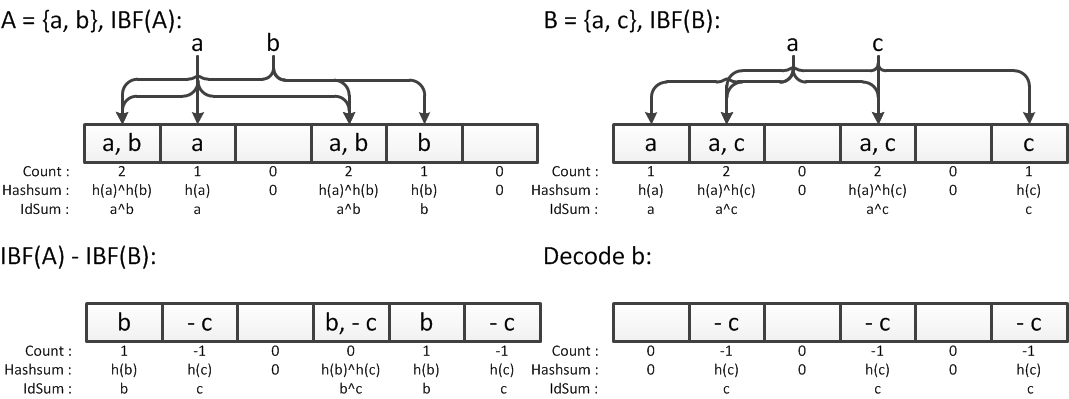
\includegraphics[width=0.9\textwidth]{InvertibleBloomFilterDemo.png}
	\caption{IBF的工作过程}
	\label{fig:IBF}
\end{figure}
\par
IBF在Bloom Filter\footnote{介绍,http://en.wikipedia.org/wiki/Bloom\_filter}的基础上为每个桶添加了和字段以及和哈希字段,并为和哈希字段提供了利用异或求和的方法,从而使得通过将两个IBF做差(同样是异或),将有较高的概率恢复出得到IBF的两个集合之间的不同。这里受到篇幅限制,无法详细描述IBF的工作流程以及大小随恢复差集的概率的关系。
\par
IBF作为对比方案,其应用体现在文中的理论分析\ref{IBFComparisonSection}部分。
\section{开发引擎Unity3D}
\par
本文开发的游戏应用采用的时Unity3D引擎。该引擎为了兼顾不同的平台,采用了DotNet架构的开源实现Mono Framework。目前该引擎仍然基于Mono 2.6\footnote{官方站点,http://www.mono-project.com/Main\_Page}版本,因此并未提供对DotNet 4.0的特性的支持。该引擎提供了从C\#,语法上类似Javascript的UnityScript,以及自定义语言Boo到IL的编译工具。本应用和为应用提供支持的开发者函数库采用的是C\#编程语言,编译链接的DotNet版本为2.0。
\par
在该游戏引擎中,游戏的对象存储在按照名称索引和组织的一棵树中。
\section{本章小结}
\par
本章描述了论文中所使用的主要技术,和其与论文设计方案、优化方案、对比方案的联系。命名数据网是设计方案基于的网络架构;已知的同步模型是本文方案的参照和对比;开发者函数库是本文工作的另一个需求和开发的基础;游戏联机技术是本文研究的对象,其IP下的实现是本文的对比;kNN问题和Digest的表示与本文的设计决定和对比方案或是优化有关系。为了帮助充分理解文章在设计方案中做出的选择和考虑,本章对CCN架构和同步模型的描述较为详细。